\chapter{Evaluation}

In this section we explain the experimental setup, experimental results and discuss the results of the several experiment conducted in detail. 

\section{Evaluation Metrics}
In this section we explain the evaluation metrics used in the experiments. In the experiments we use commonly used evaluation metrics like, sensitivity, specificity, accuracy, roc curve. Table ~\ref{tab:configs} shows the possible outcomes of the experiments conducted. True positives are the number of truly detected subjects as abnormal, false negatives are the abnormal subjects but detected as normal by the test. Similarly true negative is number of truly detected subjects as being normal and false positives are subjects that are normal but classified as abnormal by the tests. Notice that depending on the experiments abnormal either means having diabetic retinopathy or having mocelar edema. Definitions of the evaluation metrics are as follows: 

\begin{align*}
    sensitivity &= \frac{TP}{TP + FN}
    &
    specificity &= \frac{TN}{TN + FP}
\end{align*}

\begin{align*}
    accuracy &= \frac{TP + TN}{TP + FP + TN + FN}
\end{align*}

\begin{table}[t]
\centering
\caption{Test subject definitions} 
\label{tab:configs}
\begin{tabular}{|c|c|c|c|} \hline
     & Abnormal & Normal & Total  \\ \hline
     Abnormal& True Positive(TP) & False Positive (FP) & TP + FP \\ \hline
     Normal & False Negative (FN) & True Negative (TN) & TN + FN \\ \hline
     Total & TP + FN &  FP + TN & TP + FN + FP + TN \\ \hline
\end{tabular}
\end{table}

\subsection{Receiver operating characteristic (ROC)}
Another evaluation metric commonly used for diabetic retinopathy research is ROC. ROC is grahical representation of the fraction of TP  vs. FP. TP rate is also known as sensitivity, and FP rate is 1 minus the specificity. 

\subsection{Log Loss}
Logistic loss that is used in neural networks, is the negative log-likelihood of the true labels given a probabilistic classifier’s predictions. For a single sample with true label yt in {0,1} and estimated probability yp that yt = 1, the log loss is
\begin{align*}
    -log P(yt|yp) = -(yt log(yp) + (1 - yt) log(1 - yp))  
\end{align*}

\section{Experimental Configuration}
We run several different experiments with different configurations. Used configurations are as follows:

\begin{itemize}
    \item Nothing: It means images are only scaled to the same size used by the training of the models (128x128 in our experiments). No histogram equalization, enhancement, contrast or rotation is applied to the images. 
    \item Rotate: Both during training and testing images are rotated randomly since in most of the data available, images can belong different eyes (left or right) and their appereance can differ. 
    \item Rotate\_Heq: After random rotation, histogram equalization is applied to all of the images. 
    \item HeqOnly: No rotation is applied to the images, only histogram equalization is used. 
    \item RotateContrast1.5: Medium level of contrast enhancement is applied to the images after random rotation.
    \item RotateContrast1.52: High level of contrast enhancement is applied to the images after random rotation.
    \item AllConf: After random rotation, contrast, sharpen and edge enhance is applied to the image.
\end{itemize}

\section{Experiments with Messidor Dataset}
We run all the experiments in this section by using k-fold cross validation with the settings of k=6. We first shuffle the dataset and split the dataset into 6 folds. Each time we use 80\% of the data as training data and 20\% as test data. We run the following experiments.

\subsection{DR vs NonDR}
Figure \ref{messidoracc} shows accuracy results for Messidor data experiments with average of 6 fold experiments. It can be observed that best configuration is using random rotaion only or AllConf. Almost with 70\% accuracy classifier can truely predict whether eye image contains signs of diabetic retinopathy or not. Table \ref{tab:msdll} shows the logloss values for the experiments. Again the smallest error is obtained by using only rotation.

\begin{figure}[!htbbp]
\centering
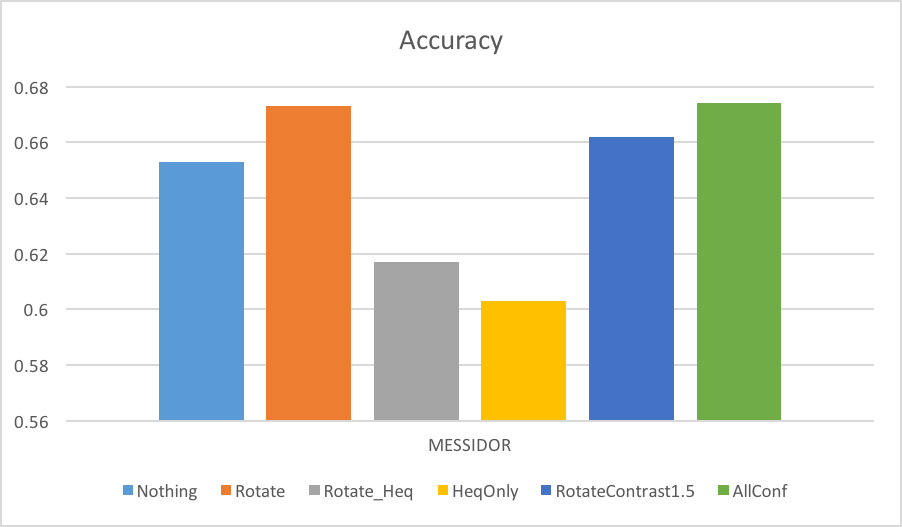
\includegraphics[width=0.8\textwidth]{Figures/messidor.png}
\caption{Accuracy results for Messidor dataset with different preprocessing steps}
\label{messidoracc}
\end{figure}

\begin{table}[t]
\centering
\caption{Messidor Dataset Log Loss values for Experiments} \label{tab:msdll}
\begin{tabular}{|c|c|c|c|c|c|c|} \hline
 & Nothing & Rotate & Rotate\_Heq & HeqOnly & RotateContrast1.5 & AllConf \\ \hline
log loss & 0.68 & 0.654 & 1.024 & 1.002 & 0.762 & 0.686 \\ \hline
\end{tabular}
\end{table}

\subsection{DR degree prediction}
This is 4 class prediciton.
\subsection{MA vs NonMA}
By looking at the results of the DR NONDR experiments, by using best performed configuration, only rotation, we run a further experiment for the detection of risk of having macular edema or not. Table \ref{tab:msdma} shows the results.  

\begin{table}[t]
\centering
\caption{Messidor Dataset Experimet Results for MA risk detection} \label{tab:msdma}
\begin{tabular}{|c|c|c|c|c|c|c|} \hline
 Accuracy & Log loss \\ \hline
 0.81 & 0.518\\ \hline
\end{tabular}
\end{table}

\section{Experiments by using other datasets}
In this section we train a convolutional neural network model by using all of the Messidor dataset as training data. 
\subsection{Stare Dataset Experiments}
In this part, we show the results of the experiments run with using Messidor dataset as traiing data and Stare dataset as test data. 93 DR and 36 NONDR data. Accuracy results are shown on Figure \ref{stareacc}. ROC graphs for Stare dataset experiments are shown on Figure \ref{stareroc}.\\
Both accuracy results and ROC graphs shows that best configuration is the raw configuration, namely Nothing. Around 70\% of accuracy is obtained and 0.7 area under ROC curve is obtained.   

\begin{figure}[!htbbp]
\centering
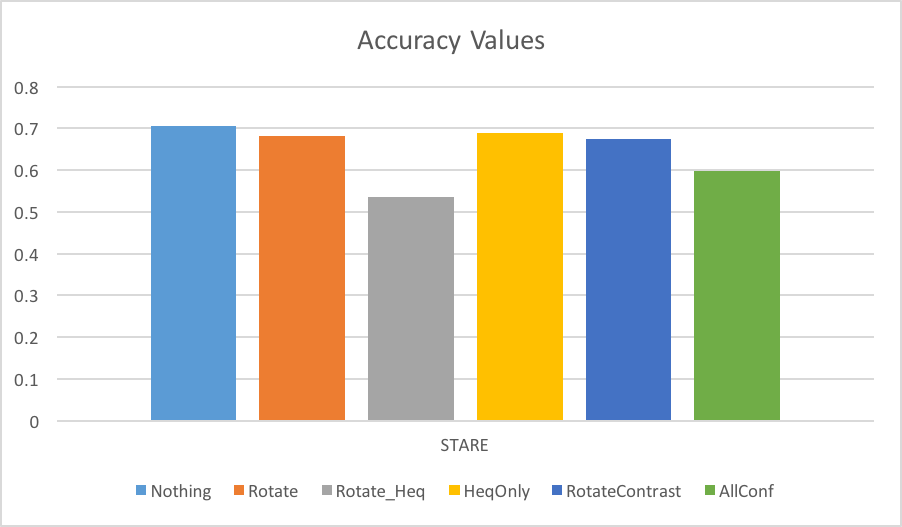
\includegraphics[width=0.8\textwidth]{Figures/stareacc.png}
\caption{Accuracy results for Stare dataset with different preprocessing steps}
\label{stareacc}
\end{figure}

\begin{figure}[!htbbp]
\centering
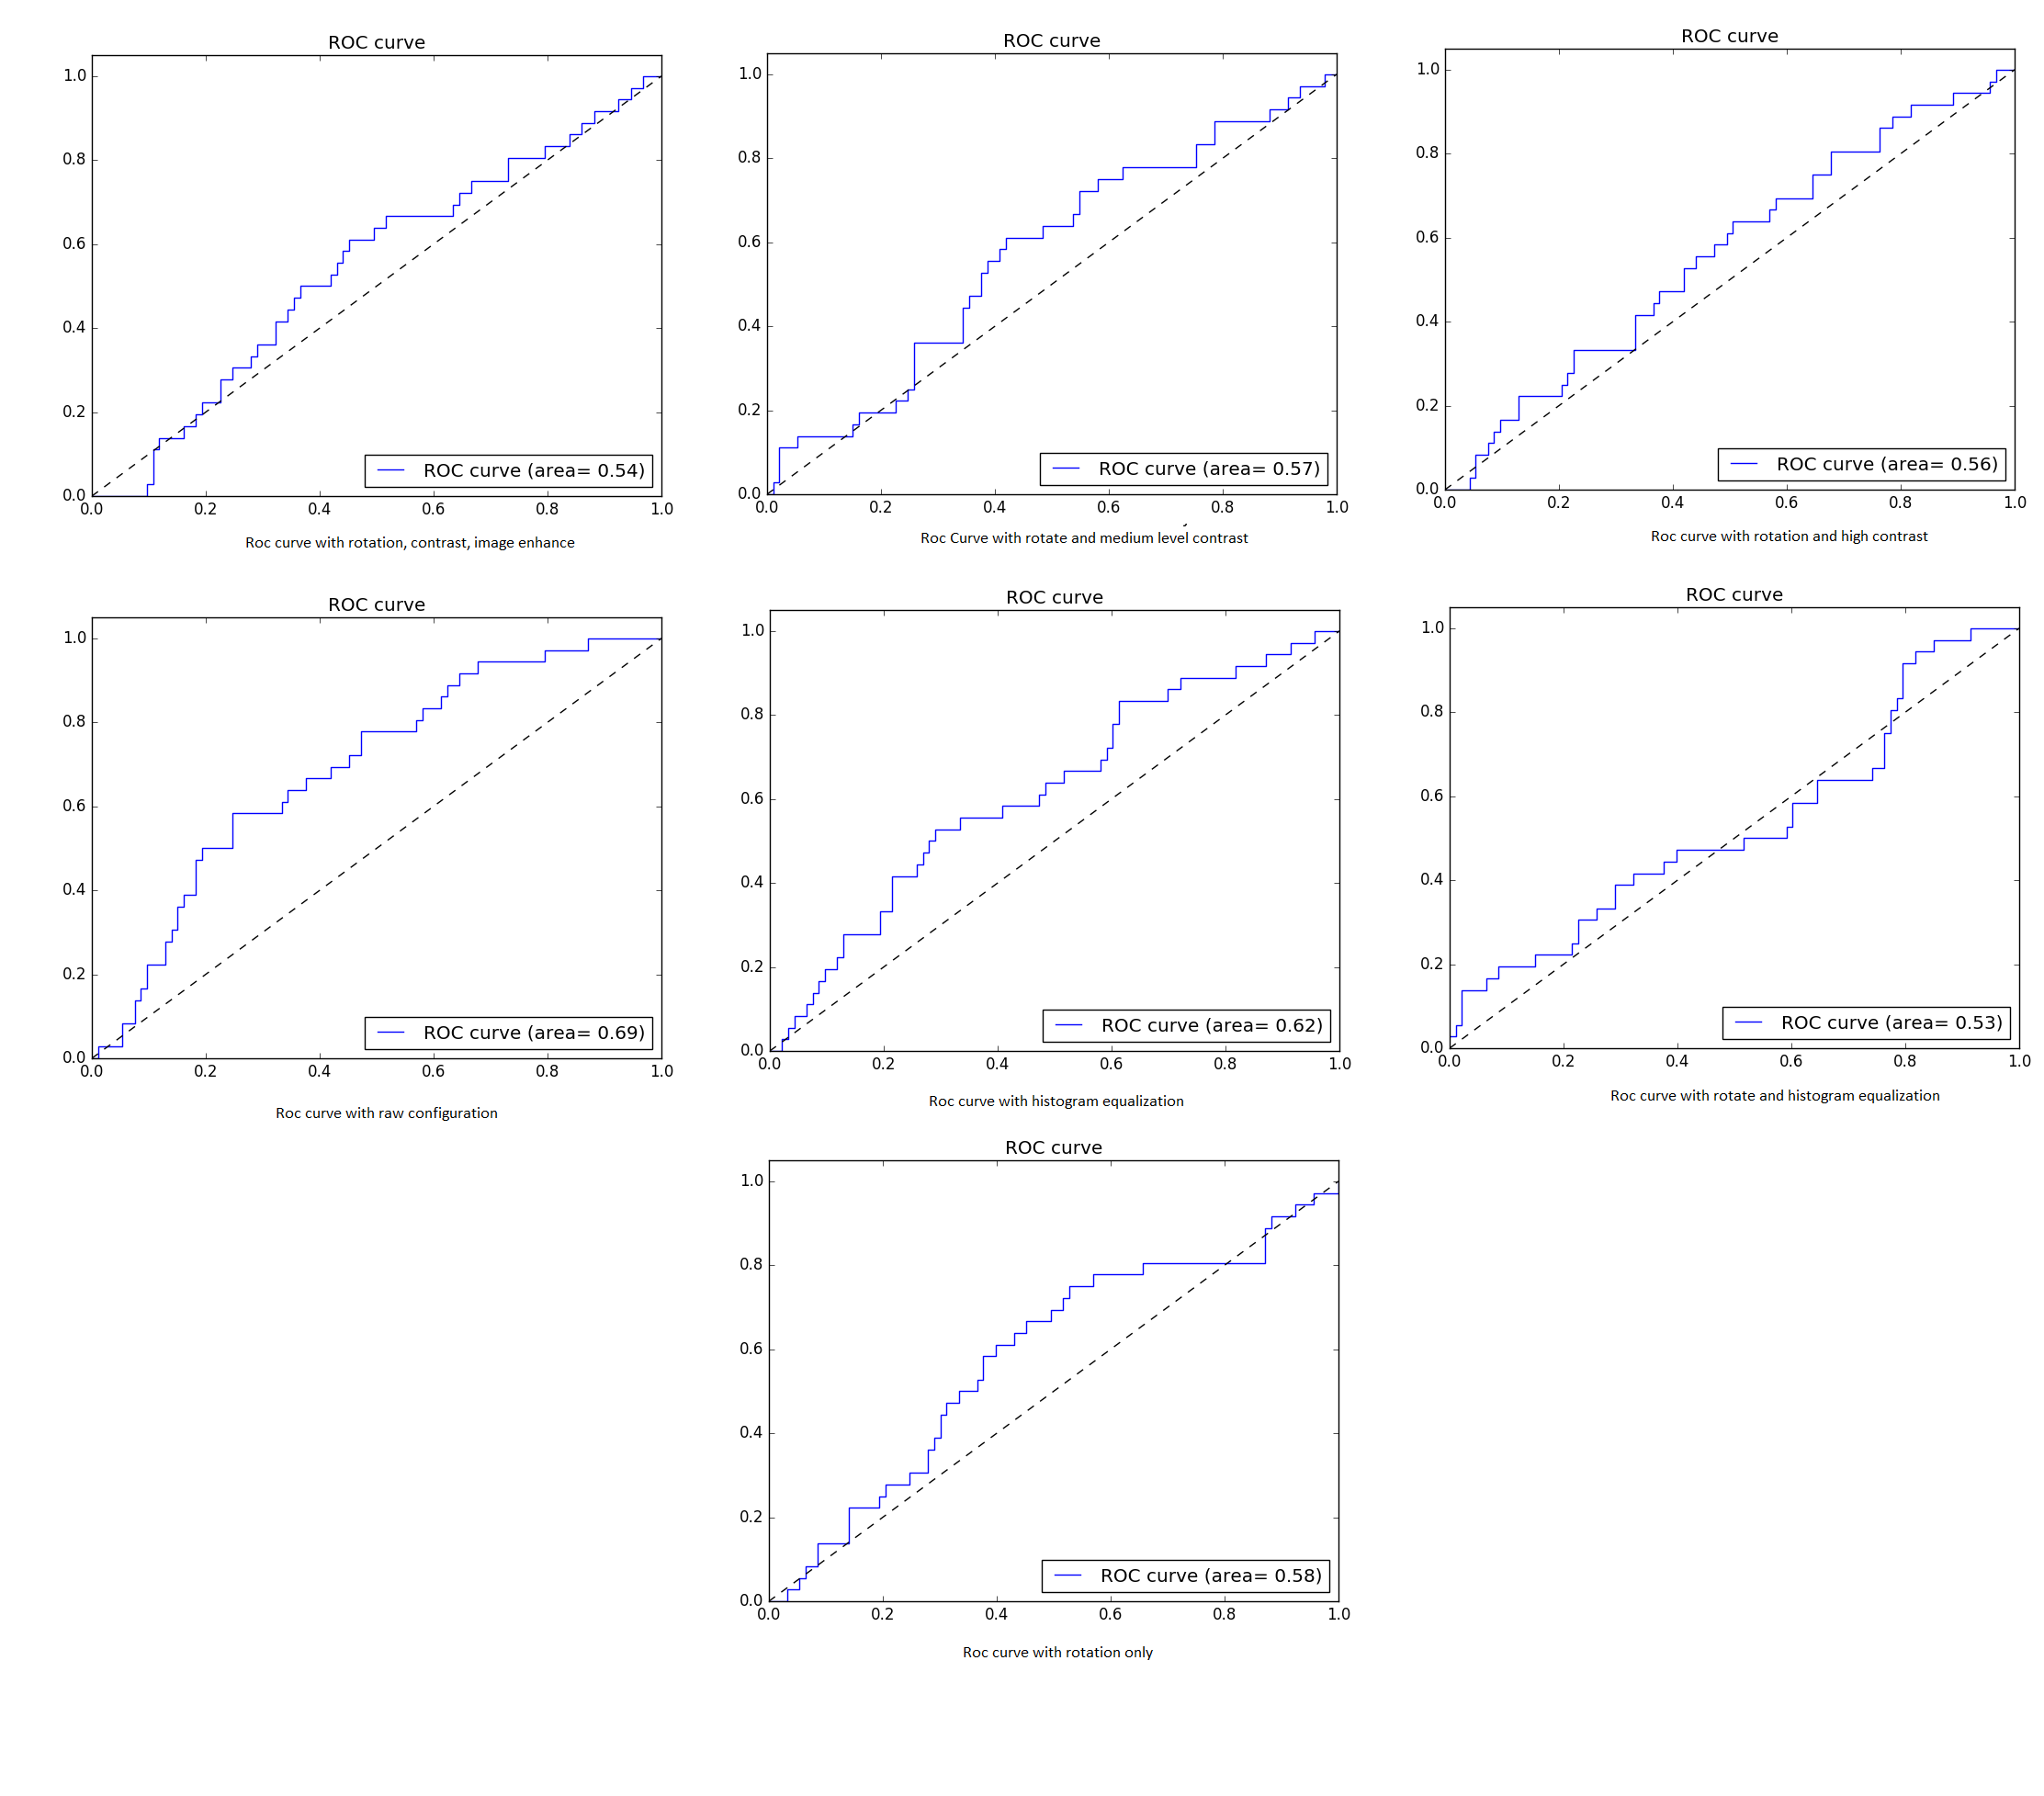
\includegraphics[width=1.0\textwidth]{Figures/stare.png}
\caption{ROC for Stare dataset with different preprocessing steps}
\label{stareroc}
\end{figure}

\subsection{Colour Fundus Images of Healthy Persons \& Patients with Diabetic Retinopathy Dataset(CFI) Experiments}
In this part, we show the results of the experiments run with using Messidor dataset as traiing data and CFI dataset \citep{alipour2012analysis} as test data. 35 DR and 25 NONDR data.\\
Accuracy results are shown on Figure \ref{cfiacc}. ROC graphs for Stare dataset experiments are shown on Figure \ref{cfiroc}.\\
By using random rotation only around 80\% of accuracy results can be obtained and 0.9 area under ROC curve can be obtained with the same configuration. This is one of the best results obtained in our experiments. 

\begin{figure}[!htbbp]
\centering
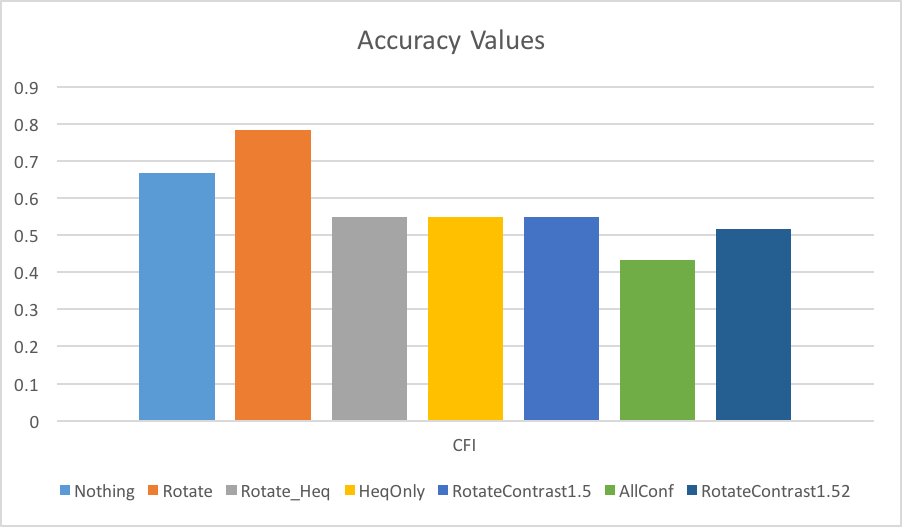
\includegraphics[width=0.8\textwidth]{Figures/cfiacc.png}
\caption{Accuracy results for CFI dataset with different preprocessing steps}
\label{cfiacc}
\end{figure}

\begin{figure}[!htbbp]
\centering
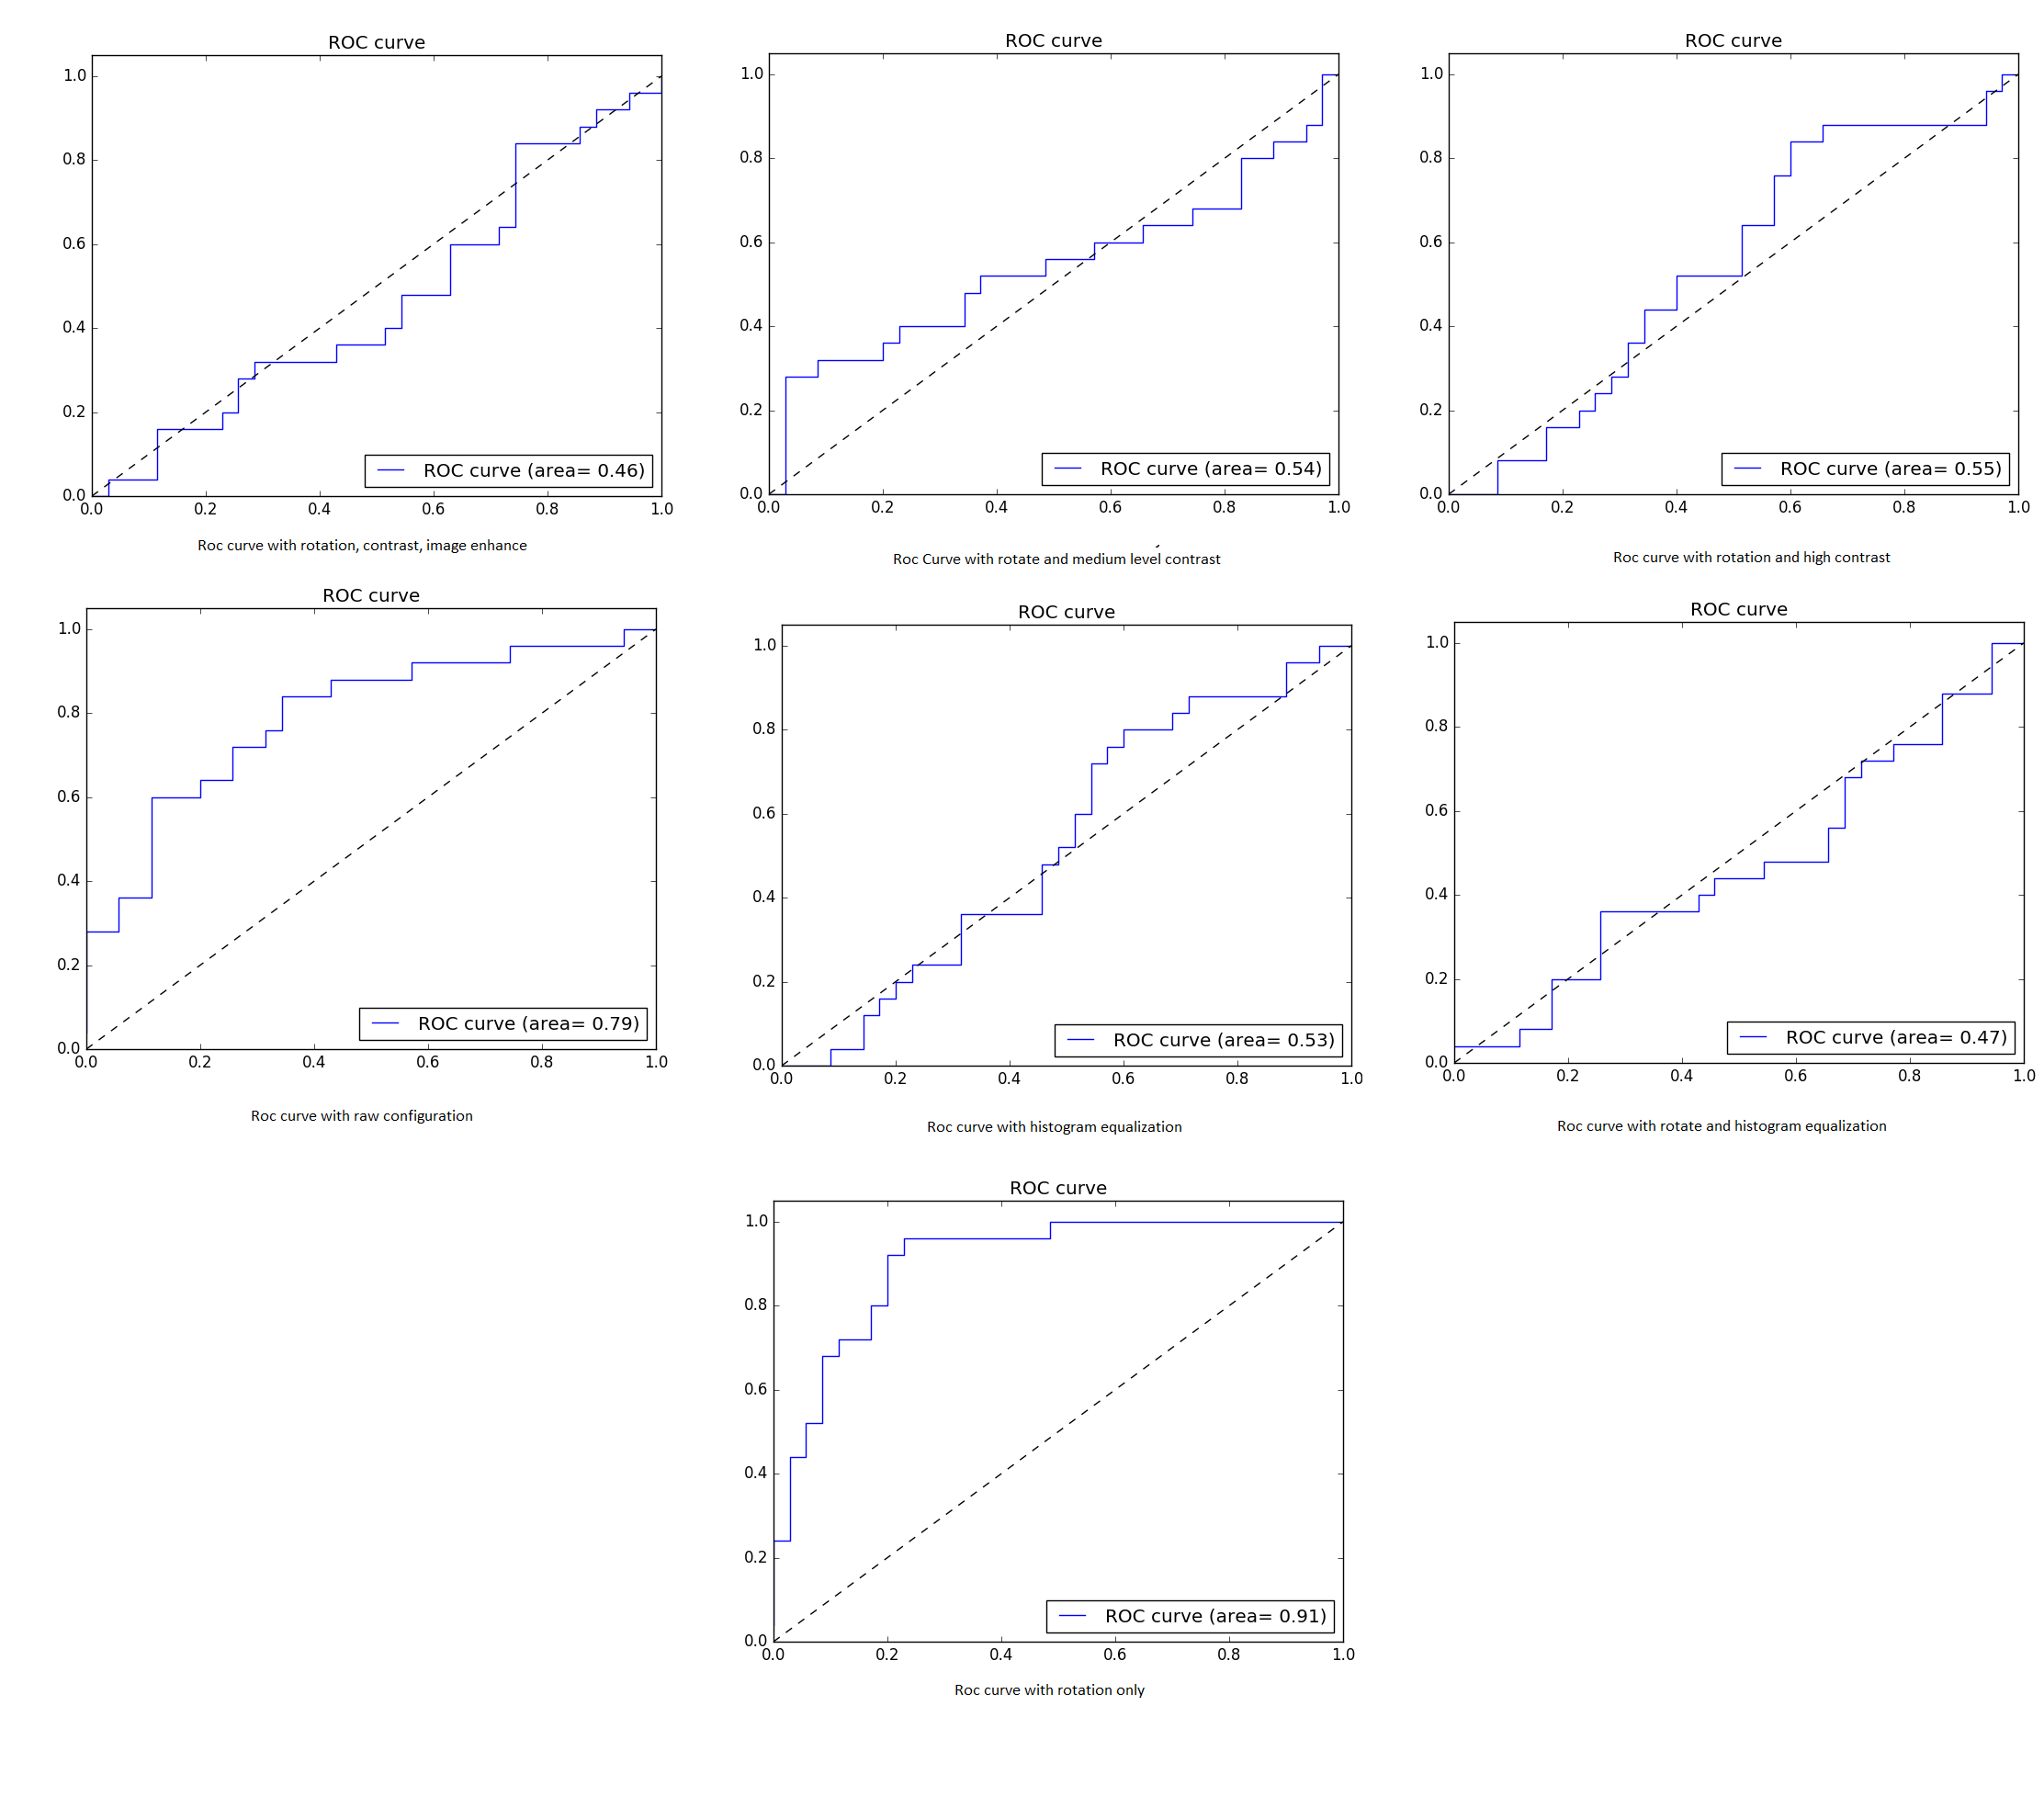
\includegraphics[width=1.0\textwidth]{Figures/cfi.png}
\caption{ROC for CFI dataset with different preprocessing steps}
\label{cfiroc}
\end{figure}


\subsection{High Resolution Fundus Dataset(HRF) Experiments}
In this part, we show the results of the experiments run with using Messidor dataset as traiing data and HRF dataset as test data. 15 DR and 15 NONDR data.\\
Accuracy results are shown on Figure \ref{hrfacc}. ROC graphs for Stare dataset experiments are shown on Figure \ref{hrfroc}.\\
By using raw configuration, applying nothing to the images, around 60\% of accuracy results can be obtained and 0.75 area under ROC curve can be obtained with applying histogram equalization to the images

\begin{figure}[!htbbp]
\centering
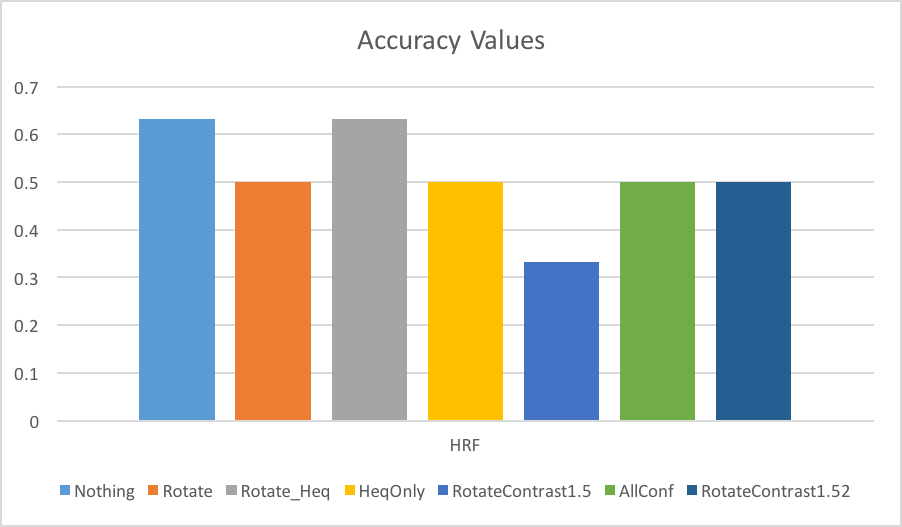
\includegraphics[width=0.8\textwidth]{Figures/hrfacc.png}
\caption{Accuracy results for HRF dataset with different preprocessing steps}
\label{hrfacc}
\end{figure}


\begin{figure}[!htbbp]
\centering
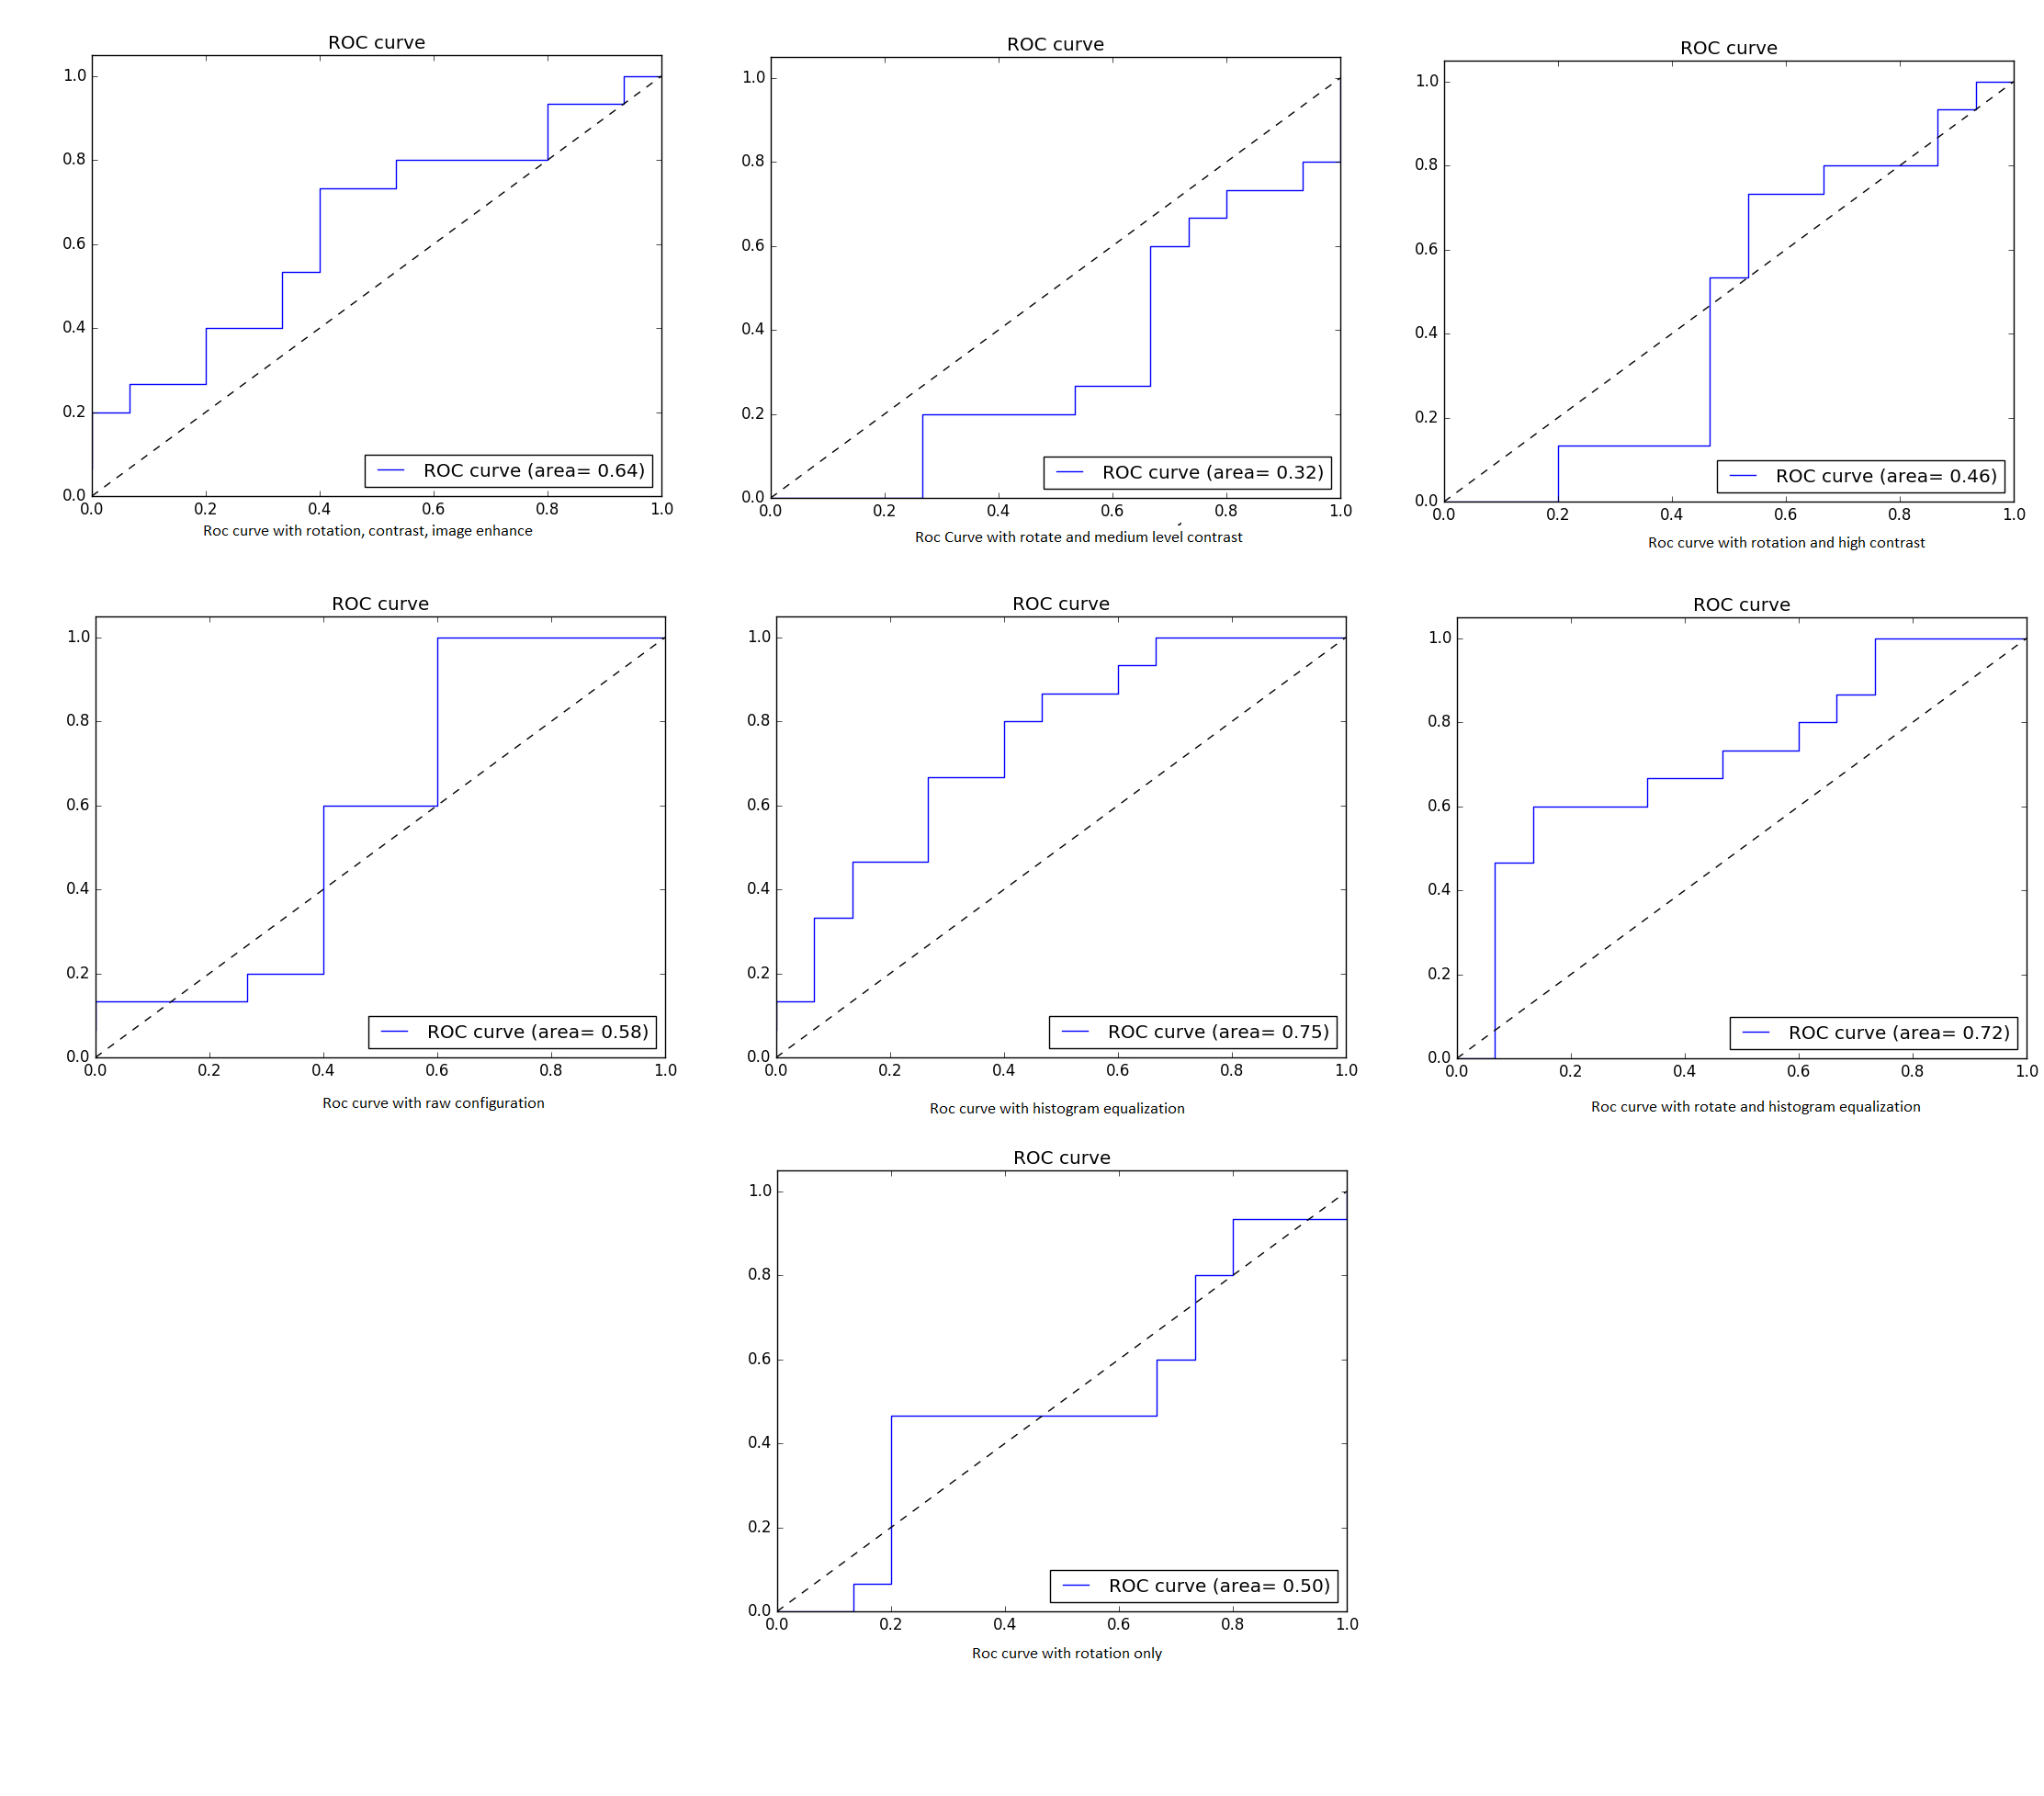
\includegraphics[width=1.0\textwidth]{Figures/hrf.png}
\caption{ROC for HRF dataset with different preprocessing steps}
\label{hrfroc}
\end{figure}